\documentclass[a4paper]{article}

\def\npart {UF PHA 6125}
\def\nterm {Module 2A/2B/2C}
\def\nyear {2026}
\def\nlecturer {Vozmediano and Cristofoletti; Rowland/Tozer; Jeong/Jusko updates}
\def\ncourse {Clearance, Distribution, and Absorption}
\def\ncoursehead {Module 2 ADME}
\def\nauthor {NanFangHong}

\RequirePackage{etex}
\makeatletter
\ifx \npart \undefined
  \def\npart{PK/PD Notes}
\fi
\ifx \nterm \undefined
  \def\nterm{Reading notes}
\fi
\ifx \nyear \undefined
  \def\nyear{\the\year}
\fi
\ifx \nlecturer \undefined
  \def\nlecturer{the source literature}
\fi
\ifx \nauthor \undefined
  \def\nauthor{NanFangHong}
\fi
\ifx \ncourse \undefined
  \def\ncourse{Pharmacology Reading Note}
\fi
\ifx \ncoursehead \undefined
  \def\ncoursehead{\ncourse}
\fi

\author{Based on \nlecturer \\\small Notes taken by \nauthor}
\date{\nterm\ \nyear}
\title{\npart\ --- \ncourse}

\usepackage{amsfonts}
\usepackage{amsmath}
\usepackage{amssymb}
\usepackage{amsthm}
\usepackage{booktabs}
\usepackage{caption}
\usepackage{enumitem}
\usepackage{fancyhdr}
\usepackage{fontspec}
\usepackage{graphicx}
\usepackage{iftex}
\usepackage{mathtools}
\usepackage{microtype}
\usepackage{siunitx}
\usepackage{tabularx}
\usepackage{tikz}
\usepackage{xcolor}
\usepackage{xurl}
\usepackage{xeCJK}

\IfFontExistsTF{Latin Modern Roman}{
  \setmainfont[Ligatures=NoCommon]{Latin Modern Roman}
}{}

\IfFontExistsTF{Noto Serif CJK SC}{
  \setCJKmainfont{Noto Serif CJK SC}
}{
  \IfFontExistsTF{Songti SC}{
    \setCJKmainfont{Songti SC}
  }{
    \IfFontExistsTF{PingFang SC}{
      \setCJKmainfont{PingFang SC}
    }{}
  }
}

\usepackage[hidelinks,unicode,breaklinks=true]{hyperref}
\hypersetup{
  pdfauthor={\nauthor},
  pdfsubject={\npart\ - \ncourse},
  pdftitle={\npart\ - \ncourse},
  pdfkeywords={PK PD pharmacology reading notes \ncourse}
}

\pagestyle{fancyplain}
\lhead{\emph{\nouppercase{\leftmark}}}
\rhead{
  \ifnum\thepage=1
  \else
    \npart\ \ncoursehead
  \fi}

\theoremstyle{definition}
\newtheorem*{aim}{Aim}
\newtheorem*{assumption}{Assumption}
\newtheorem*{defi}{Definition}
\newtheorem*{eg}{Example}
\newtheorem*{notation}{Notation}
\newtheorem*{question}{Question}
\newtheorem*{remark}{Remark}
\newtheorem*{warning}{Warning}

\theoremstyle{plain}
\newtheorem{nthm}{Theorem}[section]
\newtheorem{nprop}[nthm]{Proposition}

\renewcommand{\labelitemi}{--}
\renewcommand{\labelitemii}{$\circ$}
\renewcommand{\labelenumi}{(\roman{*})}

\let\stdsection\section
\renewcommand\section{\newpage\stdsection}

\newcommand{\dd}{\mathop{}\!\mathrm{d}}
\newcommand{\Emax}{E_{\max}}
\newcommand{\pksym}[1]{\ifmmode\text{\textit{#1}}\else\textit{#1}\fi}
\newcommand{\pklab}[1]{\mathrm{#1}}
\newcommand{\ECfifty}{\pksym{EC}_{50}}
\newcommand{\term}[1]{\emph{#1}}
\makeatother

\title{\npart\ --- Clearance, Distribution,\\ and Absorption}
\author{Based on UF PHA 6125 Module 2\\\small Rowland/Tozer and Jeong/Jusko updates\\\small Notes taken by NanFangHong}
\usetikzlibrary{arrows.meta,positioning,calc,shapes.geometric,decorations.pathreplacing,fit}
\emergencystretch=4em
\sloppy
\captionsetup{width=0.9\textwidth, justification=raggedright, singlelinecheck=false}
\lhead{\emph{\npart}}
\rhead{\ncoursehead}

\DeclareMathOperator*{\argmin}{arg\,min}
\newcommand{\Prob}{\mathbb{P}}
\newcommand{\Ex}{\mathbb{E}}
\newcommand{\given}{\,|\,}
\newcommand{\rv}[1]{\mathsf{#1}}
\newcommand{\CL}{\ensuremath{\pksym{CL}}}
\newcommand{\CLR}{\ensuremath{\pksym{CL}_{R}}}
\newcommand{\CLH}{\ensuremath{\pksym{CL}_{H}}}
\newcommand{\CLB}{\ensuremath{\pksym{CL}_{B}}}
\newcommand{\CLp}{\ensuremath{\pksym{CL}_{p}}}
\newcommand{\CLu}{\ensuremath{\pksym{CL}_{u}}}
\newcommand{\CLint}{\ensuremath{\pksym{CL}_{\pklab{int}}}}
\newcommand{\CLbile}{\ensuremath{\pksym{CL}_{\pklab{bile}}}}
\newcommand{\Vd}{\ensuremath{\pksym{V}_d}}
\newcommand{\Vss}{\ensuremath{\pksym{V}_{ss}}}
\newcommand{\AUC}{\ensuremath{\pksym{AUC}}}
\newcommand{\AUMC}{\ensuremath{\pksym{AUMC}}}
\newcommand{\Cmax}{\ensuremath{C_{\pklab{max}}}}
\newcommand{\Tmax}{\ensuremath{T_{\pklab{max}}}}
\newcommand{\Fa}{\ensuremath{\pksym{F}_a}}
\newcommand{\Fg}{\ensuremath{\pksym{F}_G}}
\newcommand{\Fh}{\ensuremath{\pksym{F}_H}}
\newcommand{\Fbio}{\ensuremath{F}}
\newcommand{\fu}{\ensuremath{f_u}}
\newcommand{\fup}{\ensuremath{f_{u,p}}}
\newcommand{\fub}{\ensuremath{f_{u,b}}}
\newcommand{\fd}{\ensuremath{f_d}}
\newcommand{\ER}{\ensuremath{\pksym{ER}}}
\newcommand{\EH}{\ensuremath{E_H}}
\newcommand{\GFR}{\ensuremath{\pksym{GFR}}}
\newcommand{\Qh}{\ensuremath{Q_H}}
\newcommand{\Qr}{\ensuremath{Q_R}}
\newcommand{\Qt}{\ensuremath{Q_T}}
\newcommand{\Rb}{\ensuremath{R_b}}
\newcommand{\Kp}{\ensuremath{K_p}}
\newcommand{\Kpss}{\ensuremath{K_{p,ss}}}
\newcommand{\PS}{\ensuremath{\pksym{PS}}}
\newcommand{\Cin}{\ensuremath{C_{\pklab{in}}}}
\newcommand{\Cout}{\ensuremath{C_{\pklab{out}}}}
\newcommand{\Cp}{\ensuremath{C_p}}
\newcommand{\Cb}{\ensuremath{C_b}}
\newcommand{\Cu}{\ensuremath{C_u}}
\newcommand{\Ct}{\ensuremath{C_T}}
\newcommand{\ka}{\ensuremath{k_a}}
\newcommand{\kel}{\ensuremath{k_{\pklab{el}}}}
\newcommand{\Km}{\ensuremath{K_m}}
\newcommand{\Vmax}{\ensuremath{V_{\max}}}
\newcommand{\EmaxLocal}{\ensuremath{E_{\max}}}
\newcommand{\ECfiftyLocal}{\ensuremath{\pksym{EC}_{50}}}
\newcommand{\PK}{\ensuremath{\pksym{PK}}}
\newcommand{\PD}{\ensuremath{\pksym{PD}}}
\newcommand{\PKPD}{\ensuremath{\pksym{PK}/\pksym{PD}}}
\newcommand{\ADME}{\ensuremath{\pksym{ADME}}}
\newcommand{\LADME}{\ensuremath{\pksym{LADME}}}
\newcommand{\PBPK}{\ensuremath{\pksym{PBPK}}}
\newcommand{\PopPK}{\ensuremath{\pksym{PopPK}}}
\newcommand{\DDI}{\ensuremath{\pksym{DDI}}}
\newcommand{\BCS}{\ensuremath{\pksym{BCS}}}
\newcommand{\CYP}{\ensuremath{\pksym{CYP}}}
\newcommand{\Pgp}{\ensuremath{\pksym{P-gp}}}
\newcommand{\OATP}{\ensuremath{\pksym{OATP}}}
\newcommand{\PEPT}{\ensuremath{\pksym{PEPT1}}}
\newcommand{\MRT}{\ensuremath{\pksym{MRT}}}

\definecolor{pkblue}{HTML}{0B3A67}
\definecolor{pkcyan}{HTML}{1D9AA7}
\definecolor{pkgreen}{HTML}{4D8B57}
\definecolor{pkred}{HTML}{C93A3A}
\definecolor{pkorange}{HTML}{D5862C}
\definecolor{pkpurple}{HTML}{6C4AA4}
\definecolor{pkgray}{HTML}{F3F5F6}
\definecolor{pkink}{HTML}{24292F}
\tikzset{
  noteBox/.style={draw=pkblue!65, fill=pkgray, rounded corners=2pt, align=center, inner sep=5pt, font=\scriptsize},
  blueBox/.style={draw=pkblue!75, fill=pkblue!5, rounded corners=2pt, align=center, inner sep=5pt, font=\scriptsize},
  greenBox/.style={draw=pkgreen!80, fill=pkgreen!7, rounded corners=2pt, align=center, inner sep=5pt, font=\scriptsize},
  orangeBox/.style={draw=pkorange!85, fill=pkorange!8, rounded corners=2pt, align=center, inner sep=5pt, font=\scriptsize},
  redBox/.style={draw=pkred!85, fill=pkred!6, rounded corners=2pt, align=center, inner sep=5pt, font=\scriptsize},
  purpleBox/.style={draw=pkpurple!75, fill=pkpurple!6, rounded corners=2pt, align=center, inner sep=5pt, font=\scriptsize},
  noteArrow/.style={-{Stealth[length=2.2mm]}, thick, draw=pkblue!85},
  weakArrow/.style={-{Stealth[length=2.0mm]}, thick, draw=pkink!55},
  noteLabel/.style={font=\footnotesize, align=center}
}

\begin{document}
\maketitle
{\small
  \noindent\textbf{Reading motive}\\
  这是 UF PHA 6125 的 Module 2 笔记。Module 2A 讲 renal and hepatic clearance，Module 2B 讲 protein binding and drug distribution，Module 2C 讲 oral drug absorption。我的目标不是把三份课件分别摘要，而是把它们改写成一张 \ADME{} 系统图：drug 如何进入 systemic circulation，如何在 plasma/tissue 之间分布，如何被 liver 和 kidney 清除，以及这些机制如何进入 dose selection, DDI, organ impairment, food effect, bioavailability, and label thinking。
  \begin{flushright}[course note]\end{flushright}

  \vspace{5pt}
  \noindent\textbf{Reader}\\
  假设读者刚学完 Module 1，对 \CL, \Vd, half-life, \Fbio{}, \PKPD{} 这些词有初步印象，但还没有真正把 physiology、protein binding、transporters、first pass、renal mechanisms 和 hepatic extraction 连起来。本笔记会尽量从读者视角解释每个公式背后的物理含义。
  \begin{flushright}[from zero]\end{flushright}

  \vspace{5pt}
  \noindent\textbf{Update}\\
  课件来自 2020 年。本笔记保留 UF PHA 6125 的教学主线，同时参考 Rowland/Tozer Chapter 5 elimination，Jeong and Jusko 关于 \fd{} 和 classical hepatic clearance models 的更新，FDA renal/hepatic impairment 与 bioavailability guidance，以及 ICH M9/M12 对 absorption、bioequivalence、DDI、transporters and enzymes 的当前监管语言。
  \begin{flushright}[2026 view]\end{flushright}
}

\tableofcontents

\section{Module Overview: ADME as One System}

\subsection{The three official module promises}

Module 2A is titled \emph{Clearance: renal and hepatic}. Its promise is to make \CL{} concrete: clearance is the volume of plasma, blood, or unbound fluid cleared of drug per unit time, and the two major elimination routes are biotransformation and excretion. Biotransformation is usually enzymatic conversion of parent drug into metabolites, mostly in the liver but also in gut, kidney, lung, skin, and plasma. Excretion is removal of intact drug through urine, bile, saliva, body fluids, or milk.

Module 2B is titled \emph{Protein binding and drug distribution}. Its promise is to explain why a measured plasma concentration is not the same thing as the amount of drug in the body or the concentration at a tissue target. Blood perfusion, plasma protein binding, tissue binding, regional pH, membrane permeability, and physicochemical properties all shape the rate and extent of distribution. \Vd{} is the proportionality between amount in body and measured blood or plasma concentration; it is not an anatomical volume.

Module 2C is titled \emph{Drug absorption}. Its promise is to explain how orally administered drug reaches systemic blood. Oral absorption is favored by the body acting as a sink: distribution and elimination keep systemic unbound concentration low, preserving a gradient across the gut wall. Gastric emptying, intestinal transit, dissolution, permeability, transporters, intestinal metabolism, hepatic first pass, degradation, and food can all alter rate and extent.

Taken together, these three modules form one statement:
\begin{quote}
\itshape
The concentration we observe in plasma is the visible trace of input, distribution, and elimination all acting at once.
\end{quote}
This matters because almost every clinical pharmacology decision is an inverse problem. We give a dose and observe concentration--time data. From that trace we infer whether a molecule is dissolving, crossing membranes, binding to proteins, entering tissues, being extracted by liver, filtered or secreted by kidney, or being changed by food, disease, genotype, or interacting drugs.

\subsection{Why the order feels strange at first}

The course presents clearance first, then distribution, then absorption. Physiologically, a tablet obviously dissolves and absorbs before it is cleared. But pedagogically, clearance first is defensible. \CL{} is the parameter that makes exposure interpretable:
\[
  \AUC_{\pklab{IV}}=\frac{D}{\CL},
  \qquad
  \AUC_{\pklab{oral}}=\frac{\Fbio D}{\CL}.
\]
If the denominator is not understood, the numerator cannot be interpreted. A low oral \AUC{} may mean poor absorption, high first pass, high systemic clearance, or some combination of all three. Module 2 therefore starts by sharpening the exit term, then comes back to the distribution space and the oral input pathway.

\begin{remark}
  I visually inspected the three original slide decks and transcript-derived flow diagrams before redrawing the figures below. The figures are not screenshots. They are compact LaTeX/TikZ reconstructions designed to survive both ordinary PDF rendering and the pdf2htmlEX HTML route used by this site.
\end{remark}

\subsection{One ADME diagram}

\begin{center}
\resizebox{0.98\textwidth}{!}{%
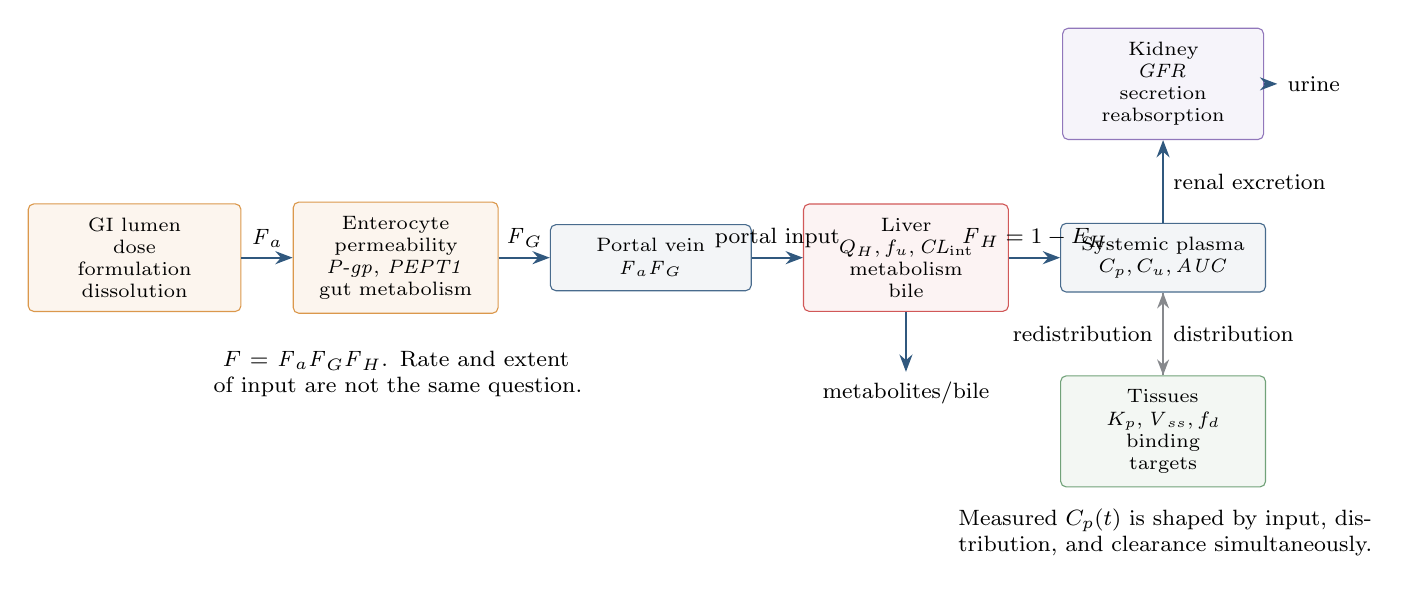
\begin{tikzpicture}[node distance=0.48cm and 0.65cm]
  \node[orangeBox, text width=2.35cm] (lumen) {GI lumen\\ dose\\ formulation\\ dissolution};
  \node[orangeBox, text width=2.25cm, right=of lumen] (enterocyte) {Enterocyte\\ permeability\\ \Pgp{}, \PEPT{}\\ gut metabolism};
  \node[blueBox, text width=2.20cm, right=of enterocyte] (portal) {Portal vein\\ \(\Fa\Fg\)};
  \node[redBox, text width=2.25cm, right=of portal] (liver) {Liver\\ \(\Qh,\fu,\CLint\)\\ metabolism\\ bile};
  \node[blueBox, text width=2.25cm, right=of liver] (plasma) {Systemic plasma\\ \(C_p,\Cu,\AUC\)};
  \node[greenBox, text width=2.25cm, below=1.05cm of plasma] (tissue) {Tissues\\ \(K_p,\Vss,\fd\)\\ binding\\ targets};
  \node[purpleBox, text width=2.20cm, above=1.05cm of plasma] (kidney) {Kidney\\ \(\GFR\)\\ secretion\\ reabsorption};

  \draw[noteArrow] (lumen) -- node[above,noteLabel]{\(\Fa\)} (enterocyte);
  \draw[noteArrow] (enterocyte) -- node[above,noteLabel]{\(\Fg\)} (portal);
  \draw[noteArrow] (portal) -- node[above,noteLabel]{portal input} (liver);
  \draw[noteArrow] (liver) -- node[above,noteLabel]{\(\Fh=1-\EH\)} (plasma);
  \draw[noteArrow] (plasma) -- node[right,noteLabel]{renal excretion} (kidney);
  \draw[noteArrow] (kidney) -- ++(1.45,0) node[right,noteLabel]{urine};
  \draw[noteArrow] (liver) -- ++(0,-1.45) node[below,noteLabel]{metabolites/bile};
  \draw[weakArrow] (plasma) -- node[right,noteLabel]{distribution} (tissue);
  \draw[weakArrow] (tissue) -- node[left,noteLabel]{redistribution} (plasma);

  \node[noteLabel, below=0.35cm of enterocyte, text width=4.8cm] (ftext) {\(\Fbio=\Fa\Fg\Fh\). Rate and extent of input are not the same question.};
  \node[noteLabel, below=0.15cm of tissue, text width=5.2cm] {Measured \(C_p(t)\) is shaped by input, distribution, and clearance simultaneously.};
\end{tikzpicture}
}
\captionof{figure}{Module 2 in one picture. The apparent simplicity of \(C_p(t)\) hides a coupled physiological system: gut input, hepatic first pass, distribution, renal clearance, hepatic clearance, protein binding, transport, and tissue partitioning.}
\end{center}

\subsection{The four concentration languages}

The same molecule can be described by several concentrations. Confusing these is the fastest way to make \PK{} formulas feel mystical.
\[
  \text{rate of elimination}
  =
  \CLp C_p
  =
  \CLB C_b
  =
  \CLu C_u.
\]
The rate is physical. The clearance value depends on the concentration used as reference. This is why Rowland/Tozer repeatedly distinguishes plasma clearance, blood clearance, and unbound clearance \cite{rowlandTozer2019ClinicalPKPD}. A clearance name is therefore a coordinate system. We should know the organ, the process, and the reference fluid:
\[
\begin{array}{lll}
  \text{organ:} & \CLH,\ \CLR,\ \CLbile, & \text{liver, kidney, bile;}\\[2pt]
  \text{process:} & \CL_{\pklab{met}},\ \CL_{\pklab{sec}},\ \CL_{\pklab{fil}}, & \text{metabolism, secretion, filtration;}\\[2pt]
  \text{fluid:} & \CLp,\ \CLB,\ \CLu, & \text{plasma, blood, unbound plasma water.}
\end{array}
\]
The warning is simple: the organ name and process name are not synonyms. In casual speech, ``hepatic clearance'' often means hepatic metabolic plasma clearance. But liver can also excrete drug into bile, and kidney can metabolize drug.

When estimating organ extraction, the denominator should be blood flow and blood concentration, not plasma flow and plasma concentration:
\[
  \CLB = Q\,E,
  \qquad
  E=\frac{\Cin-\Cout}{\Cin}.
\]
If only plasma clearance is reported, a blood clearance can be obtained from the plasma-to-blood concentration ratio:
\[
  \CLB = \CLp\frac{C_p}{C_b}.
\]
This correction is not decorative. A drug with a high plasma clearance may still have a low hepatic extraction ratio if much of the drug resides in plasma rather than whole blood, or if the plasma-to-blood ratio is unusual because of red-cell partitioning or plasma-protein binding. The symbol \(\CL\) is therefore incomplete unless we know whether it is plasma-based, blood-based, unbound, renal, hepatic, biliary, systemic, or apparent after oral dosing.

\section[2A: Renal and Hepatic Clearance]{2A: Clearance}

\subsection{Clearance is a proportionality, not a bucket}

The safest definition is:
\[
  \text{rate of elimination}
  =
  \CL \times C.
\]
If \(C\) is plasma concentration, \(\CL\) is plasma clearance; if \(C\) is blood concentration, \(\CL\) is blood clearance; if \(C\) is unbound concentration, \(\CL\) is unbound clearance. The unit is volume per time, but no literal volume of plasma is scooped out and washed clean. Clearance is a conversion factor between concentration and elimination rate.

For linear first-order elimination, \(\CL\) is constant:
\[
  -\frac{\dd A}{\dd t}
  =
  \CL\,C.
\]
For a one-compartment IV bolus with \(C=A/\Vd\),
\[
  \frac{\dd C}{\dd t}
  =
  -\frac{\CL}{\Vd}C
  =
  -\kel C,
  \qquad
  t_{1/2}=\frac{\log 2}{\kel}=\frac{\log 2\,\Vd}{\CL}.
\]
This is the key Module 1 connection: half-life is not a primary elimination capacity. It is the consequence of \CL{} and \Vd{}.

\subsection{First-order, zero-order, and capacity-limited elimination}

The Module 2A objectives ask for first-order and zero-order elimination. These are not just curve shapes.

\begin{itemize}[leftmargin=2em]
  \item \textbf{First-order elimination}: a constant fraction of the amount is removed per unit time. Rate increases in proportion to concentration. \(\CL\) is constant.
  \item \textbf{Zero-order elimination}: a constant amount is removed per unit time. Rate is approximately independent of concentration. Apparent \(\CL=\text{rate}/C\) decreases as concentration increases.
  \item \textbf{Michaelis--Menten elimination}: the mechanistic bridge between the two:
  \[
    \text{rate}
    =
    \frac{\Vmax C}{\Km+C}.
  \]
  When \(C\ll\Km\), rate \(\approx(\Vmax/\Km)C\), so elimination looks first-order. When \(C\gg\Km\), rate \(\approx\Vmax\), so elimination looks zero-order.
\end{itemize}

The clinical point is that a dose increase can be harmless under linear elimination and dangerous under saturable elimination. The parameter \(\AUC\) no longer scales linearly with dose once \(\CL\) becomes concentration-dependent.

\subsection{Intrinsic clearance lives inside the cell}

Clearance is measured outside the organ, usually from plasma or blood data. But elimination occurs at a cellular site: an enzyme, transporter, or excretory surface. Rowland/Tozer use \(\CLint\) for this intrinsic eliminating activity. Conceptually,
\[
  \text{rate of elimination}
  =
  \CLint\,C_{u,\pklab{cell}},
\]
where \(C_{u,\pklab{cell}}\) is the unbound concentration available to the intracellular enzyme or transporter. If several primary hepatic pathways operate in parallel, intrinsic clearance is additive:
\[
  \CLint
  =
  \sum_j \CL_{\pklab{int},j}
  =
  \CL_{\pklab{int,met}}
  +
  \CL_{\pklab{int,ex}}
  +
  \cdots.
\]
This sounds like a small notational detail, but it is a conceptual guardrail. Plasma concentration is what we measure; intracellular unbound concentration is often what the eliminating machinery sees. The two are close only if binding equilibrium, membrane permeation, and transport are fast enough relative to blood transit through the organ.

\subsection{Mass balance across an organ}

For a clearing organ at steady state, the input rate is \(Q\Cin\) and the output rate is \(Q\Cout\). The amount removed per time is
\[
  Q(\Cin-\Cout).
\]
Dividing by \(Q\Cin\) gives extraction ratio:
\[
  E=\frac{Q(\Cin-\Cout)}{Q\Cin}
   =\frac{\Cin-\Cout}{\Cin}.
\]
Dividing the elimination rate by inlet blood concentration gives organ blood clearance:
\[
  \CLB = Q\,E.
\]
So the maximum possible blood clearance of an organ is its blood flow. This statement is simple but powerful. It tells us why high-extraction drugs are flow-limited: if the organ already removes almost everything delivered to it, increasing enzyme activity cannot extract much more than everything.

\begin{center}
\resizebox{0.82\textwidth}{!}{%
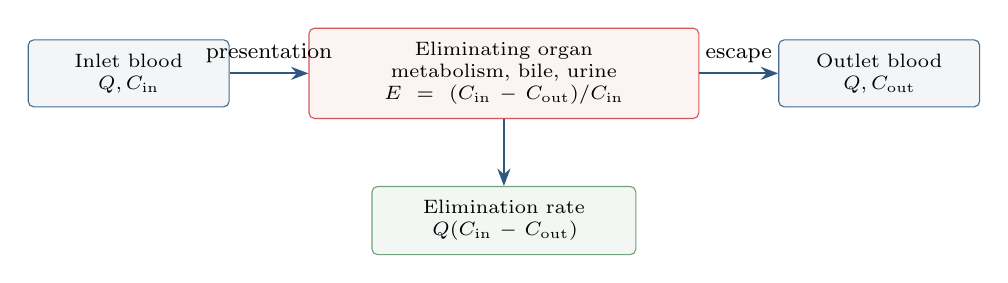
\begin{tikzpicture}[node distance=0.65cm]
  \node[blueBox, text width=2.2cm] (in) {Inlet blood\\ \(Q,\Cin\)};
  \node[redBox, text width=4.6cm, right=1.0cm of in] (organ) {Eliminating organ\\ metabolism, bile, urine\\ \(E=(\Cin-\Cout)/\Cin\)};
  \node[blueBox, text width=2.2cm, right=1.0cm of organ] (out) {Outlet blood\\ \(Q,\Cout\)};
  \node[greenBox, text width=3.0cm, below=0.85cm of organ] (elim) {Elimination rate\\ \(Q(\Cin-\Cout)\)};

  \draw[noteArrow] (in) -- node[above,noteLabel]{presentation} (organ);
  \draw[noteArrow] (organ) -- node[above,noteLabel]{escape} (out);
  \draw[noteArrow] (organ) -- (elim);
\end{tikzpicture}
}
\captionof{figure}{Organ clearance is a mass-balance idea. The extraction ratio is a fraction; blood clearance is blood flow times that fraction.}
\end{center}

\subsection{Total clearance is additive}

If a drug is eliminated by several independent routes, rates add:
\[
  \text{rate}_{\pklab{total}}
  =
  \text{rate}_{R}
  +
  \text{rate}_{H}
  +
  \cdots.
\]
For the same reference concentration, clearances add:
\[
  \CL = \CLR+\CLH+\cdots.
\]
This is why the fraction excreted unchanged in urine is so useful:
\[
  f_e=\frac{\CLR}{\CL}.
\]
If \(f_e\) is large, renal impairment can matter directly. If \(f_e\) is small, renal impairment can still matter indirectly through changes in transporters, metabolites, protein binding, or nonrenal clearance, but the first-order suspicion is different.

\subsection{Renal clearance: filtration, secretion, reabsorption}

Renal clearance decomposes into three processes:
\[
  \text{excretion}
  =
  \text{filtration}
  +
  \text{secretion}
  -
  \text{reabsorption}.
\]
Rowland/Tozer's Chapter 5 makes the bookkeeping slightly more precise. Filtration and secretion add drug to the tubular lumen; reabsorption removes some fraction of that luminal drug back into blood. If \(F_R\) denotes the fraction reabsorbed from the lumen, then
\[
  \text{rate of urinary excretion}
  =
  (1-F_R)
  \left(
    \text{rate of filtration}
    +
    \text{rate of secretion}
  \right),
\]
and, after dividing by plasma concentration,
\[
  \CLR
  =
  (1-F_R)
  \left(
    \CL_{\pklab{fil}}
    +
    \CL_{\pklab{sec}}
  \right).
\]
This form is helpful because it reminds us that \(\CLR\) is a net result. A drug can be filtered, secreted, and reabsorbed at the same time; the measured clearance only tells us which influence wins.

Only unbound drug is freely filtered at the glomerulus, so filtration clearance is
\[
  \CL_{\pklab{filtration}}
  =
  \fu\,\GFR.
\]
In a typical adult, \(\GFR\) is around \(120\)--\(130\ \pklab{mL/min}\), while renal blood flow is much larger, around \(1.1\ \pklab{L/min}\) \cite{rowlandTozer2019ClinicalPKPD,ufPha6125Module2A2020}. Therefore:
\[
  \CLR \approx \fu\GFR
  \quad\Rightarrow\quad
  \text{filtration-dominated};
\]
\[
  \CLR > \fu\GFR
  \quad\Rightarrow\quad
  \text{net active secretion};
\]
\[
  \CLR < \fu\GFR
  \quad\Rightarrow\quad
  \text{net reabsorption}.
\]
This diagnostic rule is one of the highest-yield pieces of renal \PK{}.

\begin{center}
\resizebox{0.94\textwidth}{!}{%
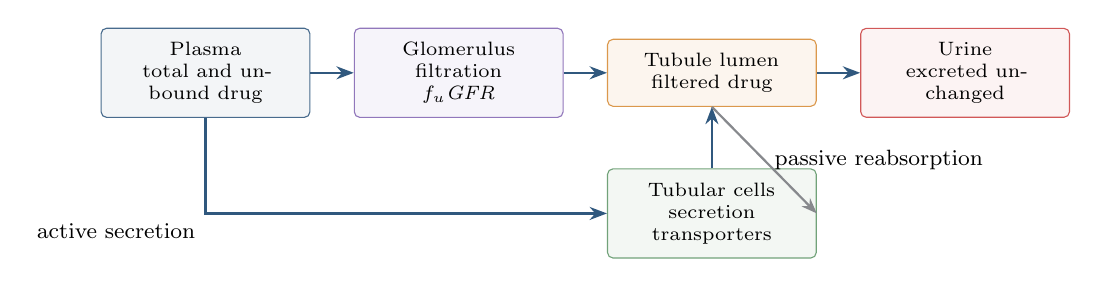
\begin{tikzpicture}[node distance=0.42cm and 0.55cm]
  \node[blueBox, text width=2.3cm] (plasma) {Plasma\\ total and unbound drug};
  \node[purpleBox, text width=2.3cm, right=of plasma] (filter) {Glomerulus\\ filtration\\ \(\fu\GFR\)};
  \node[orangeBox, text width=2.3cm, right=of filter] (tubule) {Tubule lumen\\ filtered drug};
  \node[greenBox, text width=2.3cm, below=0.78cm of tubule] (cells) {Tubular cells\\ secretion\\ transporters};
  \node[redBox, text width=2.3cm, right=of tubule] (urine) {Urine\\ excreted unchanged};

  \draw[noteArrow] (plasma) -- (filter);
  \draw[noteArrow] (filter) -- (tubule);
  \draw[noteArrow] (tubule) -- (urine);
  \draw[noteArrow] (plasma.south) |- node[below left,noteLabel]{active secretion} (cells.west);
  \draw[noteArrow] (cells) -- (tubule);
  \draw[weakArrow] (tubule.south) -- node[right,noteLabel]{passive reabsorption} (cells.east);
\end{tikzpicture}
}
\captionof{figure}{Renal clearance is not just filtration. Tubular secretion can make \(\CLR\) exceed \(\fu\GFR\); reabsorption can make it smaller.}
\end{center}

\subsection{Urine pH and urine flow}

Passive reabsorption depends on whether drug is unionized and membrane-permeable in the tubular lumen. Weak bases become more ionized at low pH and are therefore less reabsorbed; their renal clearance can increase when urine becomes acidic. Weak acids become more ionized at high pH and are therefore less reabsorbed; their renal clearance can increase when urine is alkalinized. This is the logic behind urine alkalinization for some weak-acid overdoses.

The Chapter 5 refinement is that pH sensitivity has boundaries. A nonpolar weak base is most likely to show marked pH-sensitive renal clearance when its \(pK_a\) is roughly \(7\)--\(12\): acid urine traps it in ionized form and reduces reabsorption. A nonpolar weak acid is most likely to show pH-sensitive renal clearance when its \(pK_a\) is roughly \(3\)--\(7.5\): alkaline urine traps it in ionized form. Outside these ranges, the drug may be essentially always ionized or always unionized over physiologic urine pH. And if the unionized molecule is still very polar, pH manipulation may not create much passive reabsorption in the first place.

Urine flow matters most when reabsorption is substantial. If a compound is hardly reabsorbed, forcing more urine cannot remove what was not returning anyway. If a compound is extensively reabsorbed, faster flow can reduce residence time for passive back-diffusion, increasing excretion \cite{rowlandTozer2019ClinicalPKPD}. Forced diuresis is therefore not a general detoxification lever. It is most rational when renal excretion is, or can become, a major elimination route and when tubular reabsorption is normally large. If metabolism is the dominant route and the renal pathway is tiny, even a large fold-increase in \(\CLR\) may barely move total \(\CL\).

\subsection{Hepatic clearance: blood flow, binding, intrinsic clearance}

The liver receives blood from the portal vein and hepatic artery. A useful adult average is \(\Qh\approx1.35\ \pklab{L/min}\) \cite{rowlandTozer2019ClinicalPKPD}. The classical well-stirred model summarizes hepatic blood clearance as
\[
  \CLH
  =
  \frac{\Qh\,\fub\,\CLint}{\Qh+\fub\,\CLint}.
\]
The corresponding extraction ratio is
\[
  \EH
  =
  \frac{\CLH}{\Qh}
  =
  \frac{\fub\,\CLint}{\Qh+\fub\,\CLint},
  \qquad
  \Fh = 1-\EH
  =
  \frac{\Qh}{\Qh+\fub\,\CLint}.
\]
This single expression contains the high-extraction/low-extraction distinction:
\[
  \fub\CLint \gg \Qh
  \quad\Rightarrow\quad
  \CLH\approx\Qh
  \quad\text{flow-limited};
\]
\[
  \fub\CLint \ll \Qh
  \quad\Rightarrow\quad
  \CLH\approx\fub\CLint
  \quad\text{capacity/binding-limited}.
\]

\begin{center}
\footnotesize
\begin{tabularx}{\textwidth}{p{0.21\textwidth}XX}
\toprule
Question & High hepatic extraction & Low hepatic extraction \\
\midrule
What limits \(\CLH\)? & Hepatic blood flow. The liver removes most drug delivered to it. & Intrinsic clearance and unbound fraction. Delivery is not the bottleneck. \\
Effect of increased blood flow & Often important. & Usually small. \\
Effect of enzyme induction & Systemic \(\CLH\) may change modestly, but oral \(\Fh\) can change strongly. & \(\CLH\) often increases substantially. \\
Effect of enzyme inhibition & \(\CLH\) may be less sensitive than \(\Fh\); first pass may change. & \(\CLH\) and \(\AUC\) can change strongly. \\
Effect of protein binding on total \(\CL\) & Often limited for IV systemic clearance. & Often important for total clearance. \\
Clinical warning & Oral bioavailability may be low and variable due to first pass. & Total concentration changes can reflect binding and intrinsic clearance changes. \\
\bottomrule
\end{tabularx}
\captionof{table}{The high/low extraction distinction is not a label to memorize. It predicts which physiological perturbation matters.}
\end{center}

\subsection{Access to the hepatocyte can be the bottleneck}

The well-stirred model is a superb memory aid, but Chapter 5 is careful about its hidden access assumption. It treats the unbound drug at the eliminating site as if it is readily supplied from blood. For many small lipophilic drugs, this is a reasonable first approximation. For more polar or larger molecules, the basolateral hepatocyte membrane and uptake transporters can become rate-limiting.

This matters for modern \PBPK{} thinking. A low hepatic extraction ratio does not always mean that enzyme capacity is intrinsically low. It may mean that drug reaches the enzyme or canalicular transporter slowly. In that case, a change in uptake transport, disease-related transporter expression, competing endogenous compounds, or a transporter-mediated \DDI{} can change observed hepatic clearance even when the metabolic enzyme itself is unchanged. This is the same intuition that makes Jeong/Jusko's \(\fd\) useful later: the effective contact between blood and eliminating tissue may be less than full perfusion.

\subsection{Phase I, Phase II, and transporters}

The course transcript frames biotransformation as chemical conversion of parent drug into a different molecule. A simple teaching split is:
\begin{itemize}[leftmargin=2em]
  \item \textbf{Phase I}: oxidation, reduction, hydrolysis. \CYP{} enzymes are central, especially \CYP{}3A, but not exclusive.
  \item \textbf{Phase II}: conjugation reactions such as glucuronidation, sulfation, acetylation, methylation, and glutathione conjugation.
\end{itemize}
This split is useful but incomplete unless transport is included. Hepatic clearance can require basolateral uptake into hepatocytes, metabolism or biliary excretion inside the cell, and canalicular efflux into bile. For polar compounds, uptake permeability or transporter capacity can be the rate-limiting step even when enzyme capacity is high. The modern question is therefore not only ``which enzyme metabolizes it?'' but:
\begin{quote}
\itshape
Which concentration drives elimination, and what barrier separates measured plasma from the eliminating site?
\end{quote}

\subsection{Biliary clearance and enterohepatic cycling}

The course overview lists excretion into bile alongside urine, saliva, body fluids, and milk. The Rowland/Tozer Chapter 5 expansion is worth making explicit because biliary excretion sits halfway between clearance, distribution, metabolism, transport, and absorption.

Biliary clearance can be written as
\[
  \CLbile
  =
  Q_{\pklab{bile}}
  \frac{C_{\pklab{bile}}}{C_p},
\]
where \(Q_{\pklab{bile}}\) is bile flow. Bile flow is small, roughly \(0.5\)--\(0.8\ \pklab{mL/min}\), so a drug whose bile concentration is similar to plasma concentration has small biliary clearance. But active canalicular secretion can concentrate drug or metabolite in bile; if the bile-to-plasma concentration ratio is very high, biliary clearance can become clinically meaningful.

The structural hints are useful but imperfect. Biliary excretion is more likely for polar compounds, actively transported compounds, and molecules or conjugates with molecular weight above roughly \(350\ \pklab{g/mol}\). Glucuronide conjugates often fit this pattern: they are polar, ionized, and large enough to be secreted efficiently into bile.

Enterohepatic cycling should not be confused with elimination. If drug or a glucuronide metabolite is secreted into bile, reaches the intestine, is converted back to parent drug by gut enzymes, and is reabsorbed, the molecule has cycled through a distribution loop. It becomes elimination only to the extent that drug or metabolite finally leaves the body in feces. This is why biliary obstruction can change half-life in different directions depending on whether the bile-intestine loop was part of the apparent distribution space or an actual route of loss.

\subsection{Induction and inhibition}

For low-extraction hepatic drugs, induction of enzymes or transporters often increases \(\CLH\), lowers \(\AUC\), and can shorten half-life if \Vd{} is unchanged. Inhibition does the reverse. For high-extraction drugs, systemic hepatic clearance after IV dosing may be buffered by blood flow; however, oral exposure can still change because \(\Fh=1-\EH\) is sensitive to first-pass extraction.

This resolves an apparent paradox. A high-extraction drug can have flow-limited systemic clearance and yet strong oral bioavailability changes after enzyme inhibition, because the oral pathway asks how much survives the first pass. A small absolute change in \(\EH\) near one can be a large relative change in \(\Fh\).

\subsection{First-pass metabolism}

Oral bioavailability decomposes as
\[
  \Fbio = \Fa\Fg\Fh,
\]
where \(\Fa\) is fraction absorbed into enterocytes, \(\Fg\) is fraction escaping gut-wall metabolism or efflux back to lumen, and \(\Fh\) is fraction escaping hepatic first pass. Module 2C returns to this expression in detail, but it belongs here too because \(\Fh\) is an extraction statement:
\[
  \Fh = 1-\EH.
\]
First pass is not a mysterious route separate from clearance. It is organ extraction applied before drug reaches systemic circulation.

\subsection{Regulatory update: organ impairment}

FDA's current renal impairment guidance was finalized in March 2024 and is intended to help sponsors decide when and how to study the effect of renal impairment on investigational-drug \PK{} and dosing \cite{fda2024renalImpairment}. FDA's hepatic impairment guidance remains the 2003 final guidance and covers \PK{} and, when relevant, \PD{} study design and labeling in hepatic impairment \cite{fda2003hepaticImpairment}. These guidances convert the textbook mechanisms into development questions:
\begin{itemize}[leftmargin=2em]
  \item Is renal or hepatic elimination a meaningful fraction of total clearance?
  \item Are active metabolites present?
  \item Does impaired organ function alter protein binding, transport, or nonrenal/nonhepatic pathways?
  \item Can exposure changes be translated into dose adjustment or contraindication language?
  \item Is the relevant endpoint total concentration, unbound concentration, exposure, response, or safety margin?
\end{itemize}
The important shift for students is that organ impairment studies are not ceremonial. They are how clearance mechanisms become label instructions.

\section{2B: Protein Binding and Drug Distribution}

\subsection{Distribution has rate and extent}

Drug distribution means reversible transfer between systemic circulation and tissues. Two questions must be separated:
\begin{itemize}[leftmargin=2em]
  \item \textbf{Rate}: how fast does drug move from blood to tissue and back?
  \item \textbf{Extent}: how much drug resides outside the measured plasma or blood space at distribution equilibrium?
\end{itemize}
Blood perfusion, capillary permeability, tissue permeability, active transport, pH gradients, and membrane properties govern rate. Lipophilicity, ionization, plasma protein binding, tissue binding, red-cell partitioning, and body composition govern extent.

The course examples make this intuitive. Highly lipophilic drugs can distribute into adipose tissue, creating large apparent volumes and long persistence. Hydrophilic drugs or large molecules may remain mostly in plasma and extracellular water. The blood-brain barrier is a special permeability boundary: it is not enough for a drug to be in blood; it must cross a protected interface.

\subsection{Volume of distribution is a proportionality}

\[
  \Vd = \frac{A_{\pklab{body}}}{C_p}.
\]
If a drug is mostly in plasma, \(C_p\) is high relative to amount, so \(\Vd\) is small. If a drug leaves plasma and binds extensively in tissue, \(C_p\) is low relative to amount, so \(\Vd\) is large. \Vd{} is therefore a statement about measurement and distribution, not anatomical size.

At steady state, a conceptual \PBPK{} expression is
\[
  \Vss
  \approx
  V_p
  +
  \sum_T V_T K_{p,T},
\]
where \(K_{p,T}\) is a tissue-to-plasma partition coefficient. This expression is not meant to be memorized as a universal formula. It says that \Vss{} is built from tissue volumes weighted by tissue partitioning.

\subsection{Protein binding: only unbound drug crosses and acts, but total drug is what we often measure}

Plasma protein binding is usually rapid, reversible, and approximately linear over therapeutic concentrations, although exceptions are clinically important. The unbound fraction is
\[
  \fu=\frac{C_u}{C_p}.
\]
The free-drug hypothesis says that unbound drug is the diffusible, pharmacologically active, filterable, and often metabolizable species. This is why \(\fu\) appears in filtration, hepatic clearance, in vitro--in vivo extrapolation, and interpretation of antimicrobial activity.

But the phrase ``only free drug matters'' can be misleading if it makes us ignore the system. Bound drug is a reservoir. Total concentration can change while unbound concentration remains almost unchanged, especially when clearance adapts to unbound concentration. Conversely, in nonlinear binding, hypoalbuminemia, uremia, critical illness, pregnancy, displacement interactions, or narrow-therapeutic-index drugs, unbound concentration may be the right measurement.

\subsection{When protein binding matters}

The distribution lecture emphasizes that plasma protein binding should be interpreted differently depending on extraction class \cite{ufPha6125Module2B2020}. In the low-extraction well-stirred approximation,
\[
  \CLH \approx \fub\CLint.
\]
Increasing \(\fub\) can increase total clearance. In high extraction,
\[
  \CLH \approx \Qh,
\]
so systemic clearance is less sensitive to \(\fub\), at least under the assumptions of perfusion-limited distribution and rapid binding equilibrium.

For steady-state IV infusion, the distinction between total and unbound concentration is essential. A change in protein binding can lower total concentration while leaving unbound concentration similar, because clearance and distribution are both referenced to unbound drug. This is one reason simple displacement-from-protein-binding stories often overpredict \DDI{} risk.

\begin{center}
\resizebox{0.88\textwidth}{!}{%
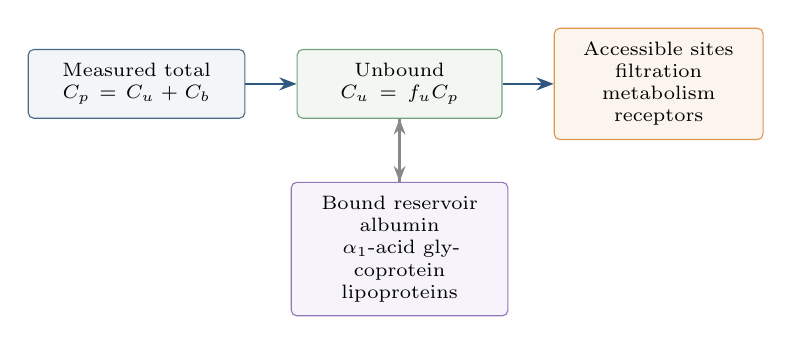
\begin{tikzpicture}[node distance=0.65cm]
  \node[blueBox, text width=2.4cm] (total) {Measured total\\ \(C_p=C_u+C_b\)};
  \node[greenBox, text width=2.25cm, right=of total] (unbound) {Unbound\\ \(C_u=\fu C_p\)};
  \node[orangeBox, text width=2.30cm, right=of unbound] (sites) {Accessible sites\\ filtration\\ metabolism\\ receptors};
  \node[purpleBox, text width=2.4cm, below=0.80cm of unbound] (bound) {Bound reservoir\\ albumin\\ \(\alpha_1\)-acid glycoprotein\\ lipoproteins};

  \draw[noteArrow] (total) -- (unbound);
  \draw[noteArrow] (unbound) -- (sites);
  \draw[weakArrow] (unbound) -- (bound);
  \draw[weakArrow] (bound) -- (unbound);
\end{tikzpicture}
}
\captionof{figure}{Protein binding links total and unbound concentration. The unbound concentration is often the pharmacological driver, but total concentration is what many assays report.}
\end{center}

\subsection{Species, methods, and nonlinear binding}

The course spends time on measurement variability because this is where pharmacology becomes experimental rather than merely algebraic. Binding can differ across species; a human \(\fu\) cannot be assumed from rat or dog. Binding can differ across assay methods such as equilibrium dialysis, ultrafiltration, and microdialysis. It can differ with albumin source, serum composition, pH, temperature, and concentration. Nonlinear binding can appear when binding sites saturate, making \(\fu\) concentration-dependent.

This matters for translation:
\begin{itemize}[leftmargin=2em]
  \item in vitro potency measured in protein-free medium may not predict in vivo potency;
  \item antimicrobial \(\pksym{MIC}\) can shift when serum is added;
  \item animal-to-human potency comparisons should often use unbound exposure;
  \item therapeutic drug monitoring may need unbound concentration for phenytoin, valproate, ceftriaxone, and selected critical-care cases.
\end{itemize}

\subsection{Distribution is not homogeneous tissue partitioning}

A visually important slide in the distribution deck warns that tissue partition coefficients are not always appropriate because they imply homogeneous tissue distribution. This is a subtle but modern point. If a drug is trapped in lysosomes, actively transported into hepatocytes, excluded from brain, or bound in a subcellular compartment, then a single \(K_p\) can be a useful empirical summary but a poor mechanism.

Azithromycin is a good example from the course: lysosomal trapping can create complex tissue distribution that cannot be reduced to ``plasma times one partition coefficient'' without losing the mechanism. In \PBPK{} language, the question becomes whether tissue is perfusion-limited, permeability-limited, transporter-limited, pH-partition-limited, or binding-limited.

\subsection{Jeong and Jusko: fractional distribution parameter fd}

Jeong and Jusko's recent work is valuable because it challenges a hidden assumption behind many classical clearance and distribution formulas: rapid perfusion-limited exchange between vascular blood and tissue \cite{jeongJusko2022Fd,jeongJusko2024Clearance}. They introduce a fractional distribution parameter \(\fd\) in \PBPK{}-style models. The product
\[
  \Qt\,\fd
\]
acts like an apparent distributional clearance into tissue. If \(\fd=1\), the tissue behaves more like a perfusion-limited compartment. If \(\fd<1\), only a fraction of delivered drug effectively crosses into tissue during a pass, reflecting permeability or uptake limitation.

Their outflow idea can be taught in words before equations:
\begin{quote}
\itshape
Blood leaving an organ is a mixture of drug that did not distribute into tissue during that pass and drug returning from tissue.
\end{quote}
A compact version is
\[
  \Cout
  =
  \Cin(1-\fd)
  +
  \frac{\Ct}{\Kp}\,\Rb\,\fd.
\]
This equation is not needed for routine noncompartmental analysis, but it is conceptually important. It says that flow \(Q\) is not always the right effective contact rate between blood and eliminating cells. Sometimes the relevant term is closer to \(Q\fd\).

\subsection{What this changes for a student}

The classical low/high extraction teaching remains useful. The update is that the student should ask more mechanistic questions before applying it blindly:
\begin{itemize}[leftmargin=2em]
  \item Is the eliminating enzyme or transporter inside a tissue compartment separated from blood by a permeability barrier?
  \item Does unbound plasma concentration equal unbound tissue concentration quickly enough?
  \item Is uptake into hepatocytes or kidney cells rate-limiting?
  \item Is measured \(K_p\) a steady-state partition coefficient, a terminal-phase tissue/plasma ratio, or a model-derived parameter?
  \item Does the organ have transit-time delay between inlet and outlet concentration?
\end{itemize}
This is the bridge from Module 2 to modern \PBPK. The equations in introductory \PK{} are not wrong; they are limiting cases of a richer transport-distribution-elimination system.

\section{2C: Drug Absorption}

\subsection{Oral absorption is rate and extent}

Oral drug delivery is common because it is convenient, scalable, and patient-friendly. But the oral route inserts a complicated system between dose and systemic exposure. The observed \(\AUC\), \(\Cmax\), and \(\Tmax\) after oral administration reflect:
\[
\begin{gathered}
  \text{formulation}
  \rightarrow
  \text{dissolution}
  \rightarrow
  \text{GI transit}
  \rightarrow
  \text{permeability/transport}
  \\
  \rightarrow
  \text{gut metabolism}
  \rightarrow
  \text{hepatic first pass}
  \rightarrow
  \text{systemic clearance}.
\end{gathered}
\]
Extent is summarized by \(\Fbio\), but rate is summarized by \(\ka\), \(\Tmax\), early exposure, or a mechanistic absorption model. A drug can have unchanged \(\AUC\) but delayed \(\Tmax\); that may matter greatly for pain relief or sleep induction and less for chronic suppression of a biomarker.

\subsection{The sink condition}

The course overview says systemic absorption is favored because the body acts as a sink. This is a beautiful way to connect absorption with distribution and clearance. If systemic unbound concentration stays low because drug distributes into tissues and is eliminated, the concentration gradient across the gut wall is maintained:
\[
  J
  =
  P\,A\,\left(C_{\pklab{lumen},u}-C_{\pklab{blood},u}\right).
\]
Here \(P\) is permeability and \(A\) is absorptive surface area. Absorption is not just a property of the gut wall. It depends on the downstream system keeping blood concentration lower than lumen concentration.

\subsection{Dissolution-limited versus permeability-limited absorption}

The Module 2C objectives ask the student to distinguish dissolution and permeability rate limitations. A practical classification is:
\begin{itemize}[leftmargin=2em]
  \item \textbf{Dissolution-limited}: drug cannot enter solution fast enough. Particle size, salt form, formulation, bile salts, and food can matter.
  \item \textbf{Solubility-limited}: drug has poor aqueous solubility; concentration in GI fluid is capped.
  \item \textbf{Permeability-limited}: drug dissolves but crosses the intestinal barrier slowly.
  \item \textbf{Transit-limited}: drug has a limited window for absorption and moves past it.
  \item \textbf{First-pass-limited}: drug enters enterocytes or portal blood but is extracted by gut wall or liver before reaching systemic circulation.
\end{itemize}

ICH M9 formalizes the \BCS{} language used in biowaivers. In vivo bioequivalence studies generally assess rate and extent using \(\AUC\) and \(\Cmax\). For appropriate immediate-release products, high solubility and permeability classifications can sometimes support waiving in vivo studies \cite{ichM9Bcs2021}. For Module 2, the pedagogical value is simple: solubility and permeability are not interchangeable.

\subsection{pH partition is useful, but not enough}

The absorption transcript uses aspirin to warn against overreading pH-partition theory. Weak acids are more unionized in acidic gastric pH, so a naive pH-partition argument predicts substantial stomach absorption. But real oral absorption also depends on dissolution, surface area, residence time, unstirred water layer, gastric emptying, intestinal permeability, and blood flow. The small intestine often dominates because it has enormous surface area and longer effective absorptive opportunity.

The rule is:
\begin{quote}
\itshape
pH and pKa tell us ionization; they do not by themselves tell us absorption.
\end{quote}

\subsection{Gastric emptying and intestinal transit}

Gastric emptying controls when dissolved or dissolving drug reaches the small intestine. Food can delay gastric emptying, change gastric pH, stimulate bile, increase splanchnic blood flow, alter viscosity, and change the migrating motor complex. For highly soluble, highly permeable drugs such as acetaminophen, food may delay \(\Tmax\) and onset without changing \(\AUC\) much. For poorly soluble lipophilic drugs, food can increase solubilization and exposure.

The course's posaconazole example illustrates positive food effect: a lipophilic, poorly soluble drug can have substantially higher oral bioavailability under fed conditions. The underlying mechanism is not simply ``food slows the stomach''. It is a formulation-solubility-bile-lipid system.

\subsection{Transporters and intestinal metabolism}

Passive diffusion is only one absorption route. Uptake transporters such as \(\OATP\), \(\PEPT\), bile-acid transporters, and monocarboxylate transporters can move drugs into enterocytes. Efflux transporters such as \(\Pgp\), \(\pksym{BCRP}\), and \(\pksym{MRP}\) can pump drug back into the lumen. Transporter-mediated kinetics can be saturable, segment-dependent, species-dependent, genotype-dependent, and susceptible to \DDI{}.

The absorption deck discusses digoxin and rifampin as a classic efflux-transporter example: induction of \(\Pgp\) can reduce oral bioavailability for \(\Pgp\) substrates. ICH M12, finalized at Step 4 in 2024, is the globally harmonized drug interaction guideline covering metabolic enzymes and transporters, including in vitro evaluation, clinical studies, predictive modeling, interpretation, and risk management \cite{ichM12Ddi2024}. This modern regulatory framing fits Module 2 exactly: absorption and clearance are not separable when gut transporters and enzymes sit in the same enterocyte.

\subsection{Bioavailability decomposition}

For an oral dose,
\[
  \Fbio=\Fa\Fg\Fh.
\]
The experimental absolute bioavailability is
\[
  \Fbio
  =
  \frac{\AUC_{\pklab{oral}}/D_{\pklab{oral}}}
       {\AUC_{\pklab{IV}}/D_{\pklab{IV}}}.
\]
FDA's 2022 bioavailability guidance covers BA information for INDs, NDAs, and supplements and specifically addresses oral dosage forms, modified-release products, and systemic exposure measures where appropriate \cite{fda2022Bioavailability}. The course formula therefore maps directly into regulatory study design: an oral \(\AUC\) is not merely an academic curve; it is evidence for formulation, food effect, dose proportionality, bridging, and label instructions.

\subsection{Saturable first-pass metabolism}

First-pass metabolism can be saturable. If gut or hepatic metabolism has a finite capacity, increasing dose may increase \(\Fbio\) because a smaller fraction is extracted. This produces nonlinear exposure:
\[
  \AUC_{\pklab{oral}}
  =
  \frac{\Fbio(D)\,D}{\CL}.
\]
Here nonlinearity can enter through \(\Fbio(D)\) even if systemic clearance after IV dosing looks linear over the same concentration range. This is one reason oral dose proportionality studies are so informative: they test the whole input-plus-clearance system.

\section{Putting 2A, 2B, and 2C Together}

\subsection{AUC, Cmax, Tmax are fingerprints of different mechanisms}

A concentration--time curve is not one parameter. Different parts of the curve report on different mechanisms:
\begin{itemize}[leftmargin=2em]
  \item \(\AUC\): extent of systemic exposure, strongly controlled by \(\Fbio D/\CL\) under linear conditions.
  \item \(\Cmax\): peak exposure, shaped by dose, \(\Fbio\), absorption rate, distribution, and clearance.
  \item \(\Tmax\): timing of peak, strongly affected by absorption rate, gastric emptying, formulation, and elimination.
  \item terminal slope: often distribution-elimination mixture; not always pure clearance.
  \item early partial \(\AUC\): important for rapid-onset indications and food/formulation assessment.
\end{itemize}
The same \(\AUC\) can hide very different early exposure; the same \(\Cmax\) can occur with different total exposure.

\subsection{Primary and secondary pharmacokinetic parameters}

One of the cleanest teaching moves in Rowland/Tozer Chapter 5 is to separate parameters closer to physiology from quantities derived from them. For Module 2, a useful working classification is:
\begin{itemize}[leftmargin=2em]
  \item \textbf{Primary disposition parameters}: \(\CLH,\ \CLR,\ \Vd,\ \Vss\).
  \item \textbf{Physiological drivers}: \(Q,\ \fu,\ \fub,\ \CLint,\ \GFR\), transport, binding, permeability, urine pH, and urine flow.
  \item \textbf{Secondary parameters or observations}: \(t_{1/2},\ \kel,\ f_e,\ \AUC,\ \Cmax,\ \Tmax\).
\end{itemize}
This distinction prevents a common interpretive reversal. A half-life does not cause clearance; half-life follows from clearance and distribution:
\[
  t_{1/2}
  =
  \frac{\log 2\,\Vd}{\CL}.
\]
Similarly, after an IV dose under linear conditions,
\[
  \AUC=\frac{D}{\CL},
  \qquad
  f_e=\frac{\CLR}{\CL}.
\]
After an oral dose,
\[
  \AUC=\frac{\Fbio D}{\CL}
  =
  \frac{\Fa\Fg\Fh D}{\CL}.
\]
So when \(\AUC\) changes, the mechanistic question is not ``what happened to \(\AUC\)?'' but which upstream determinant changed: dose, \(\Fa\), \(\Fg\), \(\Fh\), or systemic \(\CL\).

\subsection{One oral dose, many possible explanations}

Suppose a patient has unexpectedly low oral \(\AUC\). Module 2 gives a differential diagnosis:
\begin{itemize}[leftmargin=2em]
  \item the drug did not dissolve;
  \item the drug degraded in the gut;
  \item gastric emptying or intestinal transit moved the drug past its absorption window;
  \item permeability was low;
  \item efflux transporters returned drug to lumen;
  \item gut-wall metabolism was high;
  \item hepatic first-pass extraction was high;
  \item systemic clearance was high;
  \item plasma protein binding or blood/plasma partition changed the measured reference concentration;
  \item sampling missed the peak or terminal phase.
\end{itemize}
The solution is not to memorize more parameters, but to ask which mechanism would change which observable.

\subsection{A compact diagnostic table}

\begin{center}
\footnotesize
\begin{tabularx}{\textwidth}{p{0.24\textwidth}XX}
\toprule
Observation & Plausible mechanism & What to check next \\
\midrule
Low oral \(\AUC\), normal IV \(\CL\) & Poor \(\Fa\), low \(\Fg\), or low \(\Fh\) & Absolute BA, mass balance, metabolite profile, transporter/enzyme data. \\
Food delays \(\Tmax\), unchanged \(\AUC\) & Gastric emptying delay & Early exposure and onset-of-action relevance. \\
Food increases \(\AUC\) & Solubilization, bile/lipid effects, formulation dependence & Fed/fasted BA, dissolution, lipophilicity, bile-salt sensitivity. \\
\(\CLR\approx \fu\GFR\) & Filtration-dominated renal clearance & Renal impairment study relevance depends on \(f_e\). \\
\(\CLR>\fu\GFR\) & Net tubular secretion & Transporter inhibition/competition, renal \DDI. \\
\(\CLR<\fu\GFR\) & Net reabsorption & Urine pH, urine flow, lipophilicity, pKa. \\
High \(\CLH\approx\Qh\) & High extraction, flow-limited systemic clearance & First-pass, hepatic blood flow, route dependence. \\
High bile-to-plasma ratio & Active biliary secretion & Canalicular transporters, glucuronides, fecal recovery, enterohepatic cycling. \\
Large \(\Vd\) & Tissue binding/partitioning or low plasma concentration & Lipophilicity, tissue \(K_p\), lysosomal trapping, RBC partition. \\
Total concentration changes but response does not & Protein binding shift with stable unbound exposure & Measure or model unbound concentration. \\
\bottomrule
\end{tabularx}
\captionof{table}{Mechanism-oriented reading of common \PK{} observations.}
\end{center}

\subsection{The Jeong/Jusko challenge to the classical picture}

Classical clearance models are teaching masterpieces because they compress physiology into tractable equations. But Jeong and Jusko point out that the compression hides assumptions \cite{jeongJusko2024Clearance}:
\begin{itemize}[leftmargin=2em]
  \item no relevant membrane barrier between vascular blood and eliminating tissue;
  \item instantaneous unbound plasma--tissue equilibrium;
  \item intrinsic clearance acts on a concentration that is treated as directly accessible from blood;
  \item transit-time delay between inlet and outlet is often not represented in closed form.
\end{itemize}
Their extended Rattle, Sieve, Tube, and Jar models can be read as modern counterparts of dispersion, series-compartment, parallel-tube, and well-stirred ideas. For this course, the philosophical lesson is enough:
\begin{quote}
\itshape
Extraction is not only about enzyme capacity and blood flow; it is also about how drug physically reaches the eliminating site.
\end{quote}
This is especially relevant for transporter substrates, polar compounds, permeability-limited tissues, and \PBPK{} applications.

\section{Worked Examples}

\subsection{Is this renal drug filtered, secreted, or reabsorbed?}

Suppose \(\fu=0.25\), \(\GFR=120\ \pklab{mL/min}\), and measured \(\CLR=75\ \pklab{mL/min}\). Filtration alone predicts
\[
  \fu\GFR
  =
  0.25\times120
  =
  30\ \pklab{mL/min}.
\]
Because \(75>30\), net secretion must contribute. If a transporter inhibitor is coadministered, \(\CLR\) may fall, exposure may increase, and the \DDI{} could be clinically relevant if renal clearance is a meaningful fraction of total clearance.

\subsection{High extraction and first pass}

Suppose \(\Qh=90\ \pklab{L/h}\), \(\fub\CLint=810\ \pklab{L/h}\). Then
\[
  \EH=\frac{810}{90+810}=0.90,
  \qquad
  \Fh=0.10.
\]
If an inhibitor halves \(\fub\CLint\) to \(405\ \pklab{L/h}\),
\[
  \EH=\frac{405}{90+405}=0.818,
  \qquad
  \Fh=0.182.
\]
Systemic hepatic clearance changes from \(81\) to \(73.6\ \pklab{L/h}\), a modest decrease, but hepatic escape after oral dosing almost doubles. This is the high-extraction oral paradox: first-pass survival can be very sensitive even when IV systemic clearance is flow-limited.

\subsection{Low extraction and protein binding}

Suppose \(\Qh=90\ \pklab{L/h}\), \(\fub=0.01\), and \(\CLint=900\ \pklab{L/h}\). Then \(\fub\CLint=9\ \pklab{L/h}\), so
\[
  \CLH=\frac{90\times9}{90+9}=8.18\ \pklab{L/h}.
\]
If disease doubles unbound fraction to \(\fub=0.02\), then \(\fub\CLint=18\), and
\[
  \CLH=\frac{90\times18}{90+18}=15.0\ \pklab{L/h}.
\]
Total clearance rises. Total concentration at the same dose may fall. The unbound concentration may not double and may even remain closer than expected after the system equilibrates. This is why total and unbound exposure need separate thinking.

\subsection{Food effect interpretation}

Suppose an oral product has unchanged \(\AUC\) but delayed \(\Tmax\) and lower \(\Cmax\) after food. A reasonable first explanation is delayed gastric emptying and slower input, not reduced extent of absorption. For a chronic antihypertensive, this may not matter; for an analgesic intended for rapid relief, it may matter clinically. If food instead increases \(\AUC\) fivefold for a lipophilic poorly soluble drug, the first suspicion shifts toward solubilization and bile/lipid-mediated dissolution or formulation effects.

\section{How to Study This Module}

\subsection{What to memorize precisely}

Memorize these:
\[
  \text{rate of elimination}=\CL C,
  \qquad
  \CLB=Q E,
  \qquad
  E=\frac{\Cin-\Cout}{\Cin}.
\]
\[
  \CLB=\CLp\frac{C_p}{C_b},
  \qquad
  \CLu=\frac{\CLp}{\fu}.
\]
\[
\begin{aligned}
  \CL_{\pklab{filtration}}&=\fu\GFR,\\
  \CLR>\fu\GFR&\Rightarrow\text{secretion},\\
  \CLR<\fu\GFR&\Rightarrow\text{reabsorption}.
\end{aligned}
\]
\[
  \CLH
  =
  \frac{\Qh\fub\CLint}{\Qh+\fub\CLint},
  \qquad
  \Fbio=\Fa\Fg\Fh.
\]
\[
  \CLbile
  =
  Q_{\pklab{bile}}\frac{C_{\pklab{bile}}}{C_p},
  \qquad
  t_{1/2}=\frac{\log 2\,\Vd}{\CL}.
\]
\[
  \Vd=\frac{A_{\pklab{body}}}{C_p},
  \qquad
  \fu=\frac{C_u}{C_p}.
\]

\subsection{What not to memorize blindly}

Do not say ``high protein binding means low clearance'' without asking extraction class and route. Do not say ``weak acids absorb in stomach'' without asking dissolution, surface area, residence time, and intestinal permeability. Do not say ``clearance is metabolism'' because renal excretion, biliary excretion, uptake transport, and blood flow can be equally important. Do not say ``large \Vd{} means drug goes everywhere''; it may mean plasma concentration is low because of a particular tissue or binding compartment.

\subsection{A personal checklist}

For every Module 2 problem, I will ask:
\begin{itemize}[leftmargin=2em]
  \item Which concentration is referenced: plasma, blood, or unbound?
  \item If I am estimating extraction, have I converted plasma clearance to blood clearance?
  \item Is the observation about rate, extent, or both?
  \item Is clearance renal, hepatic, biliary, metabolic, excretory, or total?
  \item Is the drug high extraction or low extraction in the relevant organ?
  \item Is access to the eliminating site limited by permeability or transport?
  \item Does protein binding change total concentration, unbound concentration, clearance, distribution, or several of these at once?
  \item Is oral exposure limited by \(\Fa\), \(\Fg\), \(\Fh\), or systemic \(\CL\)?
  \item Is bile a route of loss, or is enterohepatic cycling returning drug to the system?
  \item Are transporters or permeability barriers between measured concentration and the eliminating site?
  \item Would the label need renal impairment, hepatic impairment, food-effect, DDI, or dose-adjustment language?
\end{itemize}

\section{Summary}

\subsection{One paragraph}

Module 2 turns \ADME{} from a mnemonic into a coupled physiological model. Clearance is the proportionality between concentration and elimination rate, but its value depends on the reference concentration, organ, and process: plasma, blood, unbound, renal, hepatic, biliary, metabolic, or excretory. Renal clearance is filtered plus secreted drug that escapes reabsorption, with \(\fu\GFR\) as the filtration benchmark and urine pH/flow mattering mainly when passive reabsorption is important. Hepatic clearance is shaped by blood flow, unbound fraction, intrinsic clearance, access to hepatocytes, transport, biliary secretion, and first pass. Distribution determines how amount becomes measured concentration, while protein binding separates total and unbound concentration. Absorption determines rate and extent of systemic input through dissolution, permeability, transporters, transit, food, gut metabolism, and hepatic first pass. Rowland/Tozer's primary-versus-secondary parameter distinction keeps the causality straight: half-life, \(\AUC\), and \(f_e\) follow from upstream physiological parameters. Jeong and Jusko's \(\fd\) update reminds us that the classical equations are limiting cases: drug must physically reach tissues and eliminating cells before intrinsic clearance can matter. This is the conceptual spine for interpreting \(\AUC\), \(\Cmax\), \(\Tmax\), organ impairment, food effects, and \DDI{} in later modules.

\bibliographystyle{plain}
\bibliography{../refs/pharmacology}

\end{document}
